\subsection*{Wi-Fi Data Link Layer}

The next layer in the OSI model is the Data Link Layer.
The Data Link Layer consists of Medium Access - and Logic Link Control functionalities.


According to \textcite{kauffels_wireless_2002}, the MAC functionalities cover network entry, authentication, and media access methods.
The author explains that every \ac{AP} send beacon frames periodically to synchronise its stations in the \ac{BSS} and that the beacon frame contains the \ac{SSID}, which identifies the \ac{BSS} or \ac{ESS} of the station. \textcite{sauter_wireless_2022} adds that a beacon frame contains a \SI{16}{\bit} - long capability information element. Each bit here signals that the \ac{AP} provides a particular function or has a specific feature.

\textcite{kauffels_wireless_2002} explains a station's network entry procedure.
A station can use the passive or the active scanning mode.
The station listens for a beacon frame in the various transmission channels in passive scanning mode.
Alternatively, a station can send a probe frame in active scanning mode.
The probe frame can either contain an already known \ac{SSID} to test the presence of the \ac{AP} or include a broadcast SSID that causes all nearby \ac{AP}s to respond.
The response of an \ac{AP} to the probe frame is the probe-response frame, which contains the same information as a beacon frame.
With the information from the beacon frame, a station can start the authentication process.

For this process, \textcite{kauffels_wireless_2002} names the two methods Open System Authentication and Shared Key Authentication.
\textcite{sauter_wireless_2022} explains that Open System Authentication is based on a device making an authentication
request to the \ac{AP}.
If the \ac{AP} answers with a positive status in the Authentication Frame,
the station is included in the \ac{BSS}.
The actual encryption and authentication are then performed by the \ac{WPA} functions.
The author points out that Shared Key Authentication is no longer used today.
\textcite{sommer_vehicular_2014} adds that the authentication process differs for the Ad-Hoc mode, where every station can
authenticate new stations.

After the authentication process, the station receives a time-synchronisation function with a timestamp, the physical layer
parameter configuration and the \ac{SSID} of the \ac{BSS} or \ac{ESS}.
The \ac{STA} can start the media access method now.

The IEEE 802.11 standard describes the two media access methods \ac{DCF} and \ac{PCF}.

\textcite{sauter_wireless_2022} explains that \ac{DCF} is based on the media access method \ac{CSMACA}.
In \ac{CSMACA}, a device willing to transmit senses in the air transmission medium for a transmitting activity.
If no other device is transmitting, the device can transmit.
In transmitting activity, the terminal must wait at least until the transmission and the \ac{IFS} are over.
Various access priorities are implemented by different \ac{IFS} lengths \cite{sommer_vehicular_2014}.

Since data transmission via the air transmission medium is very vulnerable to errors,
the standard IEEE 802.11 requires that each received unicast packet be confirmed with an \ac{ACK} frame \cite{sommer_vehicular_2014}.

The \ac{DCF} \ac{IFS} ensures that an \ac{ACK} frame can be sent before another station uses the same channel to send a data frame.
Each ready-to-transmit device determines
a random backoff time from a time interval called the contention window.
The device with the shortest backoff time transmits next, and all other ready-to-transmit devices restart the media access procedure to avoid multiple devices transmitting simultaneously after \ac{DIFS}.
If two devices start sending next because they randomly chose the shortest backoff time,
the transmitted signal will interfere, and the packets will not be answered with an \ac{ACK} frame.
\textcite{sommer_vehicular_2014} adds that in case of such a faulty transmission, the contention window increases exponentially until the maximum value of retries is reached and
the contention window size is reset to the starting value.

To share the knowledge of a transmission time and the subsequently \ac{IFS}, a packet contains a \ac{NAV} that
specifies the time the air transmission medium is used.
Collisions can occur as the \ac{NAV} information can be reset by other transmissions from a different, overlapping network.
To avoid this, IEEE 802.11ax maintains two \ac{NAV}s, one for intra-\ac{BSS} and one for inter-\ac{BSS} transmissions \cite{noauthor_ieee_2021}

The extension IEEE 802.11e introduced a amendment of \ac{CSMACA} called \ac{EDCA} \cite{sommer_vehicular_2014} \cite{wu_ieee_2006}.
According to \textcite{sommer_vehicular_2014}, \ac{EDCA} provides a Quality-of-Service transmission procedure, which classifies \num{4} access categories.
Each access category has a different minimum and maximum contention window sizes and different \ac{IFS} lengths, named
arbitration \ac{IFS}.
\textcite{wu_ieee_2006} explains that each access category keeps its own backoff counter and frame queue.
Every access category is handled as an independent virtual station which tries to access the medium.
When two transmissions of different access categories collide, and both contention windows are set to zero simultaneously, the \ac{EDCA} mechanism ensures that the access category with the higher priority wins.

The four access categories are listed in \autoref{tab:access_categories}.

\ac{EDCA} is integrated into the modern IEEE 802.11 standard data link layer of IEEE 802.11ac\cite{noauthor_ieee_2021-1} and IEEE 802.11ax \cite{noauthor_ieee_2021}.

\begin{table}[!ht]
   \centering
   \begin{tabular}{>{\raggedright}p{2.5cm}p{3.2cm}}
      \toprule
      Access Category & Priority (1 = Highest)\\
      \midrule
      Voice & 1 \\
      Video & 2 \\
      Best Effort & 3 \\
      Background & 4 \\
      \bottomrule
   \end{tabular}
   \caption{Access Categories and their priorities for IEEE 802.11e \ac{EDCA} \cite{wu_ieee_2006}}
   \label{tab:access_categories}
\end{table}

In various network architectures, the "hidden station"-problem may occur.
As you can see in \autoref{fig:hidden_station}, Station A cannot sense a transmission of station B and vice versa.
In case of simultaneous transmission of both stations, interferences around the \ac{AP} may occur.
\begin{figure}%
   \centering
   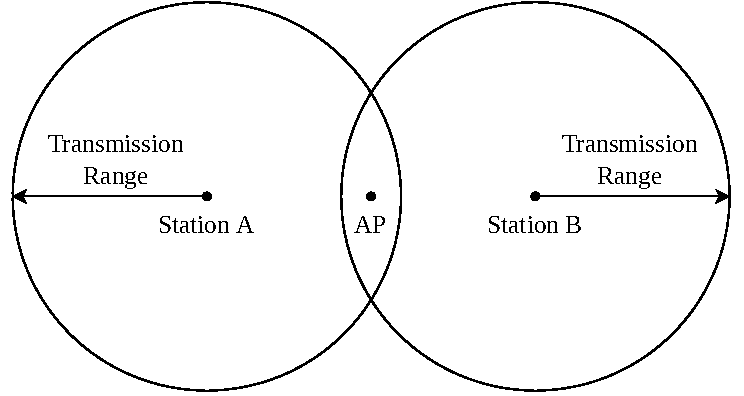
\includegraphics[width=0.75\textwidth]{figures/hidden_station.pdf}
   \caption{Hidden Station Problem, where interferences at the \acf{AP} can occur, when \acf{STA} A and B send simultaneously}%
   \label{fig:hidden_station}%
\end{figure}


To prevent the hidden station problem, \textcite{sauter_wireless_2022} explains that a \ac{STA} can access the medium
via the point coordination function.
The \ac{STA} sends a \ac{RTS} frame to the \ac{AP} and waits for a \ac{CTS} frame.
After receiving the \ac{CTS} frame, the \ac{STA} has reserved the medium for a specific time and can send its data frame.
The successful transmission of the data frame is confirmed with an \ac{ACK} frame.
To avoid another \ac{STA} accessing the medium during the \ac{RTS} and \ac{CTS} frames, the \ac{PCF} \ac{IFS} is
shorter than the \ac{DCF} \ac{IFS}.
This mechanism allows the \ac{AP} to send the \ac{CTS} frame before another \ac{STA} can access the medium.

\textcite{sauter_wireless_2022} states that the point coordination function is usually not configured because it introduces additional
overhead of the \ac{RTS} and \ac{CTS} frames, which is only worth it when the data frame is large.

Larger frames can also be split into smaller frames to reduce the probability of collisions.
This procedure, called fragmentation, divides the data into up to \num{16} frames
when a specific data length threshold is exceeded \cite{noauthor_ieee_2021}.
The fragmented frames are transmitted by the three following different \ac{ACK} policies in \autoref{fig:ACKS}, which are described by \textcite{sauter_wireless_2022}.

Using the standard \ac{ACK} policy, the sender applies the \ac{DCF} mechanism before sending each frame.
The sender also waits
for an \ac{ACK} frame from the receiver after each transmission.

Instead of operating in the \ac{DCF} mode, the sender
can also send the next frame after waiting for the \ac{SIFS} time when the \ac{ACK} frame has been received.
This is displayed in \autoref{fig:Fragmentation} and saves the overhead of acquiring the medium again.

Additional transmission time can be saved using the Block \ac{ACK} policy, shown in \autoref{fig:BLOCKACK}.
The sender sends the first frame and waits for the \ac{ACK} frame.
After transmitting all fragments, the sender sends the Block \ac{ACK} request.
The receiver sends the Block \ac{ACK} frame, which contains the information of all received frames.
Any missing frames are retransmitted.
The Block \ac{ACK} frame can be sent delayed when some processing time is required.

Every Block \ac{ACK} session is started with an add Block Acknowledgment (ADDBA) request frame, which is sent by the sender and
contains the session parameters.
The receiver sends an \ac{ACK} and answers with an add Block Acknowledgment (ADDBA) response frame.
After the sender acknowledges the response frame, the Block \ac{ACK} session is established.
The Block \ac{ACK} session is ended with a delete Block Acknowledgment (DELBA) frame, which is sent by the sender and acknowledged by the receiver.

The Block \ac{ACK} policy can be used in IEEE 802.11n \cite{noauthor_ieee_2021-1}, IEEE 802.11ac \cite{noauthor_ieee_2021-1} and IEEE 802.11ax \cite{noauthor_ieee_2021}.
In the IEEE 802.11p standard, the Block \ac{ACK} policy can be added as an optional feature \cite{noauthor_ieee_2021-1}.

\begin{figure}%
    \centering
    \subfloat[normal ACK]{\label{fig:ACK}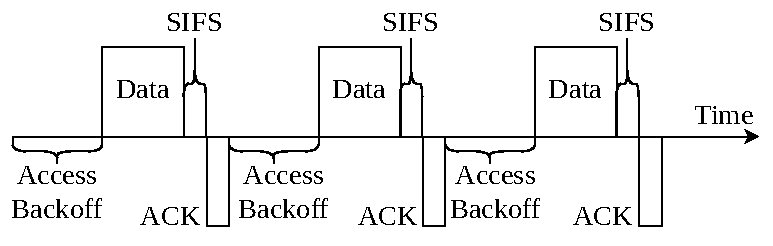
\includegraphics[width=0.7\textwidth]{figures/normalACKs}}%
    \\
    \subfloat[fragmentation]{\label{fig:Fragmentation}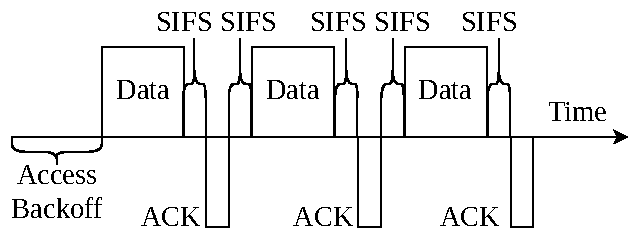
\includegraphics[width=0.7\textwidth]{figures/fragmentation}}%
    \\
    \subfloat[fragmentation and Block ACK]{\label{fig:BLOCKACK}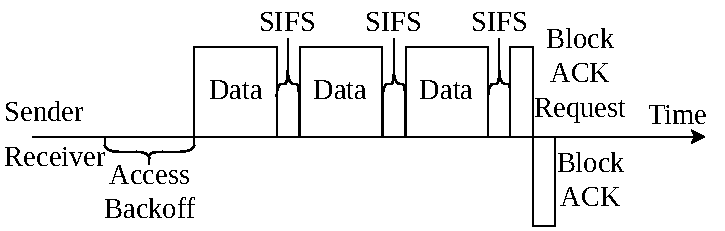
\includegraphics[width=0.7\textwidth]{figures/BlockACK}}
    \caption{Data transmission between a sender and receiver in regards to the time with normal \acf{ACK} \autoref{fig:ACK},
    fragmentation \autoref{fig:Fragmentation} and additional Block \ac{ACK} \autoref{fig:BLOCKACK}}%
    \label{fig:ACKS}%
\end{figure}



\begin{comment}
	CF Parameter set-element


MAC Header


    \cite{khorov_tutorial_2019}
Power Management Modes
Enhanced Time TWT Enhanced Microsleep

Spatial Reuse
Adaptive Power and Sensitivity Thresholds, BSS COlor

Quiet Period

Midamble Preamble


more levels of fragmentation

\end{comment}

